\textbf{{性质}{1}{:}}非空二叉树上叶子结点数等于双分支结点数加1。设度为i的结点个数为ni。性质1等式表示即为:n0=n2+1。

\textbf{{性质}{2}{:}}二叉树的第i层上最多有2\textsuperscript{i-1}个结点(i≥1)

\textbf{{性质}{3}{:}}高度为k的二叉树最多有2\textsuperscript{k}-1个结点(k≥1)。

\textbf{{性质}{4}{:}}有n个结点的完全二叉树,对各结点从上到下从左到有依次编号(1~n),则结点之间有如下关系:

若i为结点a的编号则:

如果i≠1,则a的双亲结点编号为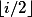
\includegraphics[width=0.33333in,height=0.17708in]{texmath/18cb1elfloori2rfloor}。

如果2×i≤n,则a有左孩子,编号为2×i,反之无左孩子。

如果2×i+1≤n,则a有右孩子,编号为2×i+1,反之无右孩子。

注:因为完全二叉树一般直接用数组存储,故通过双亲关系计算出下标的操作对完全二叉树来说是很重要的。

\textbf{{性质}{5}{:}}给定{n}个结点,能构造出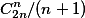
\includegraphics[width=0.88542in,height=0.18750in]{texmath/3fa64cC2nn(n+1)}{种}不同的二叉树。

\textbf{{性质}{6}{:}}具有{n}个结点的完全二叉树的深度{k}为
\textsubscript{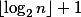
\includegraphics[width=0.84375in,height=0.17708in]{texmath/d2f760lfloorloglimitsrm2nrfloor+1}}或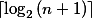
\includegraphics[width=0.95833in,height=0.18750in]{texmath/417732lceilloglimitsrm2(n+1)rceil}。
